\setcounter{page}{1}
\section*{Einleitung}
Das Verhalten von makroskopischen Vielteilchensystemen und einzelnen Atomen weist im Allgemeinen starke Unterschiede auf. Systeme, die eine Teilchenzahl zwischen einigen hundert und hunderttausend Atomen aufweisen, bilden den Übergang zwischen makroskopischem und mikroskopischem Verhalten. Die Untersuchung der optischen Eigenschaften solcher mesoskopischen Systeme hat für die Grundlagenforschung und die Technik eine hohe Relevanz und steht daher im Mittelpunkt des durchgeführten Versuchs. \cite{anleitung} \cite{bayreuth}\\
Um diese Eigenschaften für metallische Nanopartikel unterschiedlicher Form und Größe zu untersuchen, wird sich des Verfahrens der Dunkelfeldmikroskopie bedient. Dieses Verfahren basiert auf der ausschließlichen Detektion des von der untersuchten Probe emittierten Streulichtes und liefert einen faszinierenden Einblick in die Welt der Nanoplasmonik. \cite{LIU}\\
\\
Das Ziel des vorgestellten Versuchs ist die Untersuchung von Gold-Nanopartikeln mit einem Dunkelfeldmikroskop und die Bestimmung der Wirkungsquerschnitte der Teilchen nach Mie- und Rayleigh-Theorie. Außerdem werden die Polarisations- und Intensitätsabhängigkeit von der Streuung untersucht.\\

\newpage

\section{Theorie}

\subsection{Plasmonen}
In metallischen Nanopartikeln ist das oberste Leitungsband nur zum Teil durch Elektronen besetzt. Diese Leitungsbandelektronen lassen sich als quasifreie Ladungsträger beschreiben und können beispielsweise durch Einstrahlen von Licht kollektiv zu Schwingungen angeregt werden. Diese kollektive Oszillation von Leitungsbandelektronen wird als Plasmon bezeichnet. Je nach Struktur des untersuchten Metalls, wird von Volumen-, Oberflächen- oder Partikelplasmonen gesprochen. Bei Strukturgrößen im Bereich von einigen zehn bis hundert Nanometern ist die Bewegung der Ladungsträger räumlich so begrenzt, dass von lokalisierten Oberflächenplasmonen gesprochen wird, die sich im Wesentlichen wie Partikelplasmonen verhalten.\\
\\
Bei genauerer Betrachtung der Bandstruktur eines Metalls wird ersichtlich, dass die Schwingung der Ladungsträger nur durch das Vorhandensein einer Vielzahl unbesetzter Leitungsbandzustände möglich ist. Die Anregung der Elektronen kann daher beliebig stark oder schwach sein, was eine Beschreibung durch ein freies Elektronengas rechtfertigt. Für lokalisierte Oberflächenplasmonen ist zur Beschreibung der Oszillation außerdem die laterale Beschränkung der Ladungsträgerbeweglichkeit zu beachten. Die Wellenfunktionen der Elektronen wird dadurch ähnlich wie bei einem quantenmechanischen Potentialtopf eingeschränkt, woraus eine Diskretisierung der Energieniveaus folgt. Da lokalisierte Oberflächenplasmonen und Partikelplasmonen aber kein Quantenphänomen sind, kann eine semiklassiche Beschreibung der ablaufenden Prozesse vorgenommen werden. \cite{anleitung}\cite{bayreuth}\\
\\
Wird ein Partikelplasmon in einem Nanopartikel optisch angeregt, kann das einstrahlende Licht das Teilchen vollständig durchdringen. Dabei regt es die Elektronen im Leitungsband in höhere Zustände an, wodurch ein Ladungsgradient innerhalb des Partikels entsteht. Die Coulomb-Anziehung zwischenden ortsfesten positiven Ionen und den Elektronen induziert eine rücktreibende Kraft die zu einer Oszillation der Ladungsträger führt. Der Vorgang ist in Abbildung ~\ref{fig:dipol} schematisch dargestellt.
\begin{figure}[H]
  \centering
  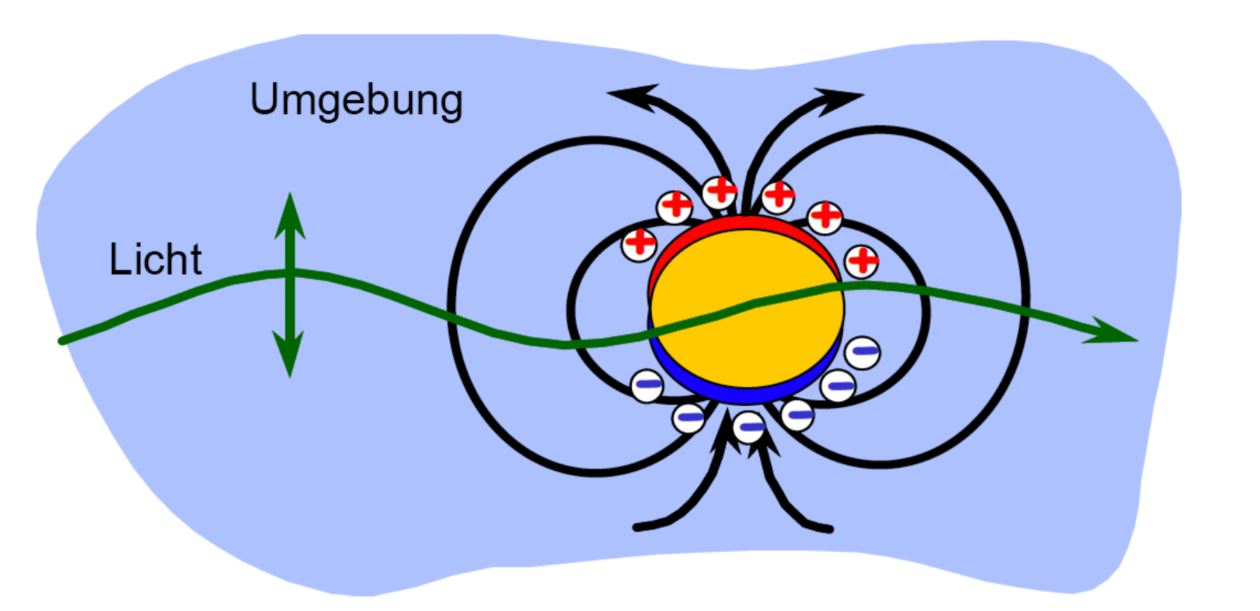
\includegraphics[width=0.8\textwidth]{plots/dipolplamson.jpg}
  \caption{Dipolmodell eines optisch angeregten Plasmons. \cite{anleitung}}
  \label{fig:dipol}
\end{figure}
Die Oszillation der Elektronen ist klassisch als ein Hertz'scher Dipol aufzufassen und strahlt dementsprechend ein elektromagnetisches Dipolfeld ab.
Werden zwei nah aneinander liegende Nanopartikel angeregt, so kommt es zur Überlagerung der beiden Dipolfelder. Diese Überlagerung führt zur sogenannten Plasmonhybridisierung, die die Energieniveaus der Schwingungen ähnlich wie bei der Orbitalhybridisierung verschiebt. Die Plasmonhybridisierung ist in Abbildung ~\ref{fig:hybrid} veranschaulicht. \cite{bayreuth} In Abbildung \ref{fig:a} ist das Feld eines einzelnen Partikelplasmons dem überlagerten Feld zweier Plasmonen gegenübergestellt. Zwischen den beiden Partikelplasmonen ist das Feld sehr stark, während es außen an den Plasmonen schwächer als bei einem einzelnen Plasmon ist. In Abbildung \ref{fig:b} ist ein Schema der Energieniveaus zweier Plasmonen zu sehen. Die einzelnen unterschiedlichen Plasmonenmoden hybridisieren zu einer symmetrischen, niederenergetischen und einer antisymmetrischen, höherenergetischen Mode.
\begin{figure}[H]
  \centering
  \begin{subfigure}{0.49\textwidth}
    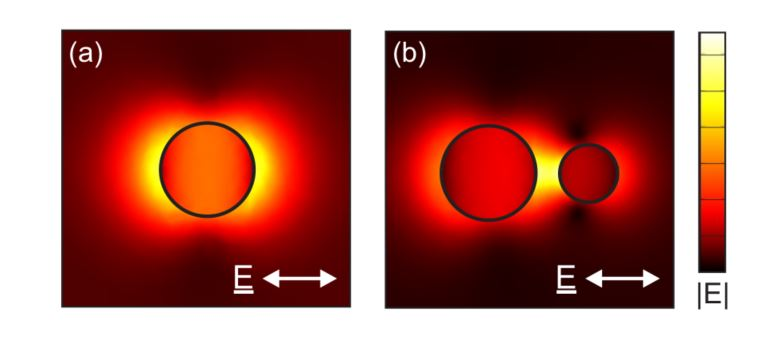
\includegraphics[width=\textwidth]{plots/hybrid.jpg}
    \caption{Einzelnes Plasmonendipolfeld (links) und überlagertes Feld zweier Plasmonen (rechts).}
    \label{fig:a}
  \end{subfigure}
  \begin{subfigure}{0.49\textwidth}
    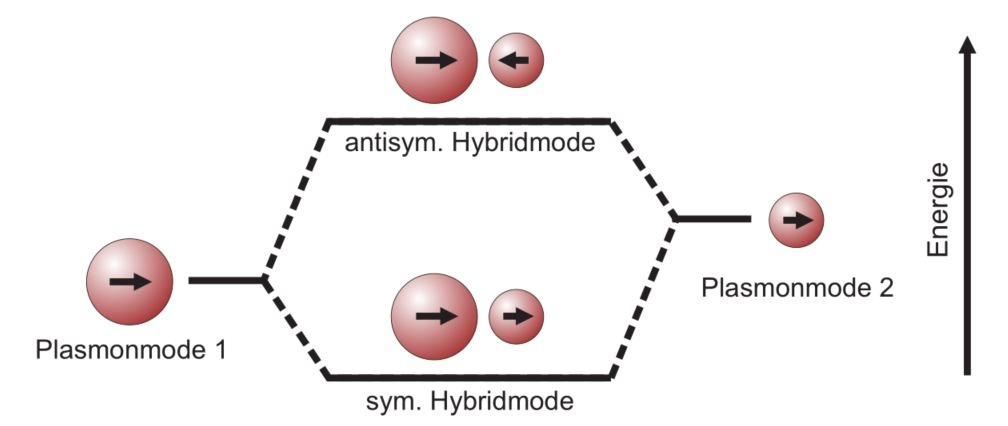
\includegraphics[width=\textwidth]{plots/hybridschema.jpg}
    \caption{Schemazeichung zweier hybridisierender Plasmonenmoden.}
    \label{fig:b}
  \end{subfigure}
  \caption{Plasmonhybridisierung zu einem symmetrischen und einem antisymmetrischen Energieniveau. \cite{bayreuth}}
  \label{fig:hybrid}
\end{figure}

\subsection{Absorption und Streuung an Plasmonen}
Bei dere Wechselwirkung von Licht mit metallischen Nanopartikeln wird zwischen Absorption in und elastischer Streuung an den beteiligten Partikeln unterschieden. Die Gesamtwechselwirkung wird durch die Extinktion quantifiziert, welche die Änderung der Transmission im Medium beschreibt.
Den drei Größen werden die Wirkungsquerschnitte $C_{\text{sc}}$, $C_{\text{abs}}$ und $C_{\text{ext}} = C_{\text{sc}} + C_{\text{abs}}$ zugeordnet.
Normierung der Wirkungsquerschnitte auf die Querschnittsfläche $A$ des Teilchens ergeben die entsprechenden Wirkungsgrade $Q_i$. Um den frequenzabhängigen Beitrag der Intensität $I$ zu Streuung, Absorption und Extinktion zu bestimmen, wird die Formel
\begin{equation}
  I_i(\omega) = \frac{I_0(\omega)}{A} C_i(\omega)
  \label{eqn:intensität}
\end{equation}
verwendet.\footnote{Der Index $i$ kann hier Wahlweise für den Absorptions-, Extinktions- oder Streuanteil stehen.} Ein weiterer aufschlussreicher Parameter ist durch die sogenannte externe Quantenausbeute
\begin{equation}
  \eta = \frac{C_{\text{sc}}}{C_{\text{ext}}} = \frac{Q_{\text{sc}}}{Q_{\text{ext}}}
\end{equation}
definiert, welche das Verhältnis von Streuung und Extinktion beschreibt. Die Parameter $C$, $Q$ und $\eta$ sind stark von der Größe des betreffenden Partikels abhängig. Für makroskopische Wechselwirkungspartner ergeben sich Wirkungsgrade von $Q_{\text{sc}} = {Q_{\text{abs}}} = 1$ und $Q_{\text{ext}} = 2$. Mit kleinerer Ausdehnung der Partikel nimmt die Streuung des Lichtes stark ab und die Absorption nimmt rapide zu.\\
\\
Die Streuung des Lichtes an den Teilchen kann aus zwei verschiedenen Theorien hergeleitet werden, welche jeweils unterschiedliche Rahmenbedingungen fordern.
\paragraph{Rayleigh-Theorie:}
In der Rayleigh-Theorie wird die Ausdehnung der Teilchen als deutlich kleiner als die Wellenlänge des eingestrahlten Lichtes angenommen. Dadurch kann die Phase der elektromagnetischen Welle über den betrachteten Raumbereich als konstant genähert werden. In der Rayleigh-Theorie kann das Teilchen als ein zu Oszillation angeregter Dipol verstanden werden, dessen Streuquerschnitt proportional zur vierten Potenz der Frequenz des Lichts ist. Aus der Herleitung des Streuquerschnitts für ein kugelförmiges Metallteilchen mit Permittivität $\epsilon_r$  und Volumen $V$ ergibt sich für die Polarisierbarkeit
\begin{equation}
  \alpha = \epsilon_0 3 V\, \frac{\epsilon_r-1}{\epsilon_r+2}\,\,.
  \label{eqn:polbarkeit}
\end{equation}
Die Streuung einer elektromagnetischen Welle mit Wellenzahl $k$ an einem solchen Teilchen führt auf die Streuquerschnitte
\begin{equation}
  C_{\text{sc}} = \frac{k^4}{6\pi}|\frac{\alpha}{\epsilon_0}|^2 \,\,\,\, \text{und}\,\,\,\, C_{\text{abs}} = k\, \symbffrak{Im}\left(\frac{\alpha}{\epsilon_0}\right)\,.
  \label{eqn:rayleigh}
\end{equation}
\paragraph{Mie-Theorie:}
In der Mie-Theorie Theorie wird die Wechselwirkung von spährischen Teilchen mit einer elektromagnetischen Welle aus den Maxwellgleichungen bestimmt. Dabei werden Teilchengrößen betrachtet, die in derselben Größenordnung wie das eingestrahlte Licht liegen. Die Maxwellgleichungen werden dazu exakt analytisch mithilfe einer Multipolentwicklung gelöst. Die erste Ordnung der Multipolentwicklung entspricht dabei einer Plasmonenresonanz, die die Rayleigh-Streuung beinhaltet. Aus den Berechnungen ergeben sich die Wirkungsgrade
\begin{equation}
  Q^{(n)}_{\text{sc}} = \frac{2}{k^2r^2} (2n+1)(|a_n^2| + |b_n^2|)
  \label{eqn:sc}
\end{equation}
\begin{equation}
  Q^{(n)}_{\text{abs}} = \frac{2}{k^2r^2} (2n+1) \symbffrak{Re}(a_n+b_n)\,.
  \label{eqn:abs}
\end{equation}
Dabei folgen aus der Entwicklung die Mie-Koeffizienten
\begin{equation}
  a_n = \frac{m\psi_n(mkr)\psi_n'(kr)-\psi_n(kr)\psi_n'(mkr)}{m\psi_n(mkr)\xi_n'(kr)-\xi_n(kr)\psi_n'(mkr)}
\end{equation}
\begin{equation}
  b_n = \frac{\psi_n(mkr)\psi_n'(kr)-m\psi_n(kr)\psi_n'(mkr)}{\psi_n(mkr)\xi_n'(kr)-m\xi_n(kr)\psi_n'(mkr)}
\end{equation}
Der Wellenvektor kann dabei durch  $k=\omega/(N_{\text{medium}}c)$ und das Verhältnis $m = N_\text{partikel}/N_\text{medium}$ der Brechungsindizes ausgedrückt werden. In die Rechnungen gehen außerdem der Partikelradius $r$, die Frequenz $\omega$ und die Riccati-Bessel-Funktionen $\psi_n$ und $\xi_n$ ein. \cite{anleitung} \cite{hoeflich}

\subsection{Einfluss von Resonanz und Dämpfung}
Die Resonanzfrequenz der Plasmonenstreuung wird durch die Rückstellkraft bestimmt. Diese hängt im Wesentlichen von der Polarisierbarkeit des Mediums und der Teilchengröße ab. Daraus folgt außerdem eine Abhängigkeit vom Umgebungsmedium, sowie von der Polarisierbarkeit der Kernelektronen.\\
\\
Um das Verhältnis zwischen Treiber- und Resonanzamplitude und die Breite der Plasmonenresonanz erklären zu können, müssen die auftretenden Dämpfungsmechanismen betrachtet werden. Die Dämpfung der Elektronenschwingung kann dabei durch stattfindende strahlende und nichtstrahlende Übergänge einzelner Elektronen in energetisch niedrigere Zustände beschrieben werden.
Die nichtstrahlende Dämpfung kann dabei ähnlich wie im Drude-Sommerfeld-Modell erklärt werden, welches ein Plasmon als Überlagerung vieler einzelner unabhängiger Elektronenschwingungen approximiert. Demnach sind wirkende Dämpfungsprozesse vor allem die Streuung an Phononen, anderen Elektronen in Kern und Hülle oder Verunreinigungen. Insgesamt wird die durch die Dämpfung verlorene Energie im Kristall in Wärme umgewandelt und geht somit verloren. \cite{anleitung}
Die Breite der Partikelplasmonresonanz ist mit den Zerfallskonstanten $\tau$ der unterschiedlichen Dämpfungsmechanismen über
\begin{equation}
  \Gamma \sim \frac{\hbar}{\tau}
\end{equation}
verbunden.\cite{sonne} Die einzelnen Zeitkonstanten sind mit den Wirkungsgraden und der strahlenden Quanteneffizienz
\begin{equation}
  \eta_{\text{rad}} = \frac{Q_{\text{sc}}}{Q_{\text{ext}}}
\end{equation}
für die Resonanzfrequenz $Q_i=Q_i(\omega_{\text{res}})$ verknüpft.
Dabei gilt
\begin{equation}
  \tau_{\text{nonrad}} \iff Q_{\text{abs}} \,\,\text{,}\,\, \tau_{\text{rad}} \iff Q_{\text{sc}} \,\,\,\, \text{und} \,\,\,\, \tau_{\text{tot}} \iff Q_{\text{ext}}.
\end{equation}
